\documentclass[12pt]{article}
\usepackage{tikz}
\usepackage{amsmath}
% Underlining package
\usepackage{ulem}
\usetikzlibrary{calc} 
\usepackage[a4paper, portrait, margin=1cm]{geometry}
\usepackage{fancyhdr}

\def \HeadingAnswers {\section*{\Large Name: \underline{\hspace{8cm}} \hfill Date: \underline{\hspace{3cm}}} \vspace{-3mm}
{Angles in Right Triangles: Answers} \vspace{1pt}\hrule}

% raise footer with page number; no header
\fancypagestyle{myfancypagestyle}{
  \fancyhf{}% clear all header and footer fields
  \renewcommand{\headrulewidth}{0pt} % no rule under header
  \fancyfoot[C] {\thepage} \setlength{\footskip}{6pt} % raise page number 6pt
}
\pagestyle{myfancypagestyle}  % apply myfancypagestyle

\newcounter{minipagecount}

\begin{document}
\HeadingAnswers
\vspace{8mm}

\begin{minipage}{0.55\textwidth}
  \refstepcounter{minipagecount}
  \noindent{(\theminipagecount)}\quad
  \begin{tikzpicture}[scale=1.5, baseline=(current bounding box.north)]
      \pgfmathsetmacro{\angleA}{36}
      \pgfmathsetmacro{\angleB}{54}
      \pgfmathsetmacro{\angleC}{90}
      \pgfmathsetmacro{\sideC}{3.9584468321061004}
      \pgfmathsetmacro{\rotationAngle}{36}
  
    
      \begin{scope}[rotate=\rotationAngle]
        \coordinate (A) at (0,0);
        \coordinate (B) at (\sideC,0);
        \coordinate (C) at (intersection cs: first line={(A)--($(A)+(\angleA:4cm)$)}, second line={(B)--($(B)+(180-\angleB:4cm)$)});
        \draw (A) -- (B) -- (C) -- cycle;
        
        % Mark angles with arcs
        \draw ($(A)!0.3cm!(B)$) arc [start angle=0, end angle=\angleA, radius=0.3cm];
        \draw ($(B)!0.3cm!(C)$) arc [start angle=180-\angleB, end angle=180, radius=0.3cm];
        % \draw ($(C)!0.3cm!(A)$) arc [start angle=180+\angleA, end angle=360-\angleB, radius=0.3cm];
        % rt angle mark at C
        % \tkzMarkRightAng0le(A,C,B); % uses \usepackage{tkz-euclide}
        \draw ($(C)!0.25cm!(A)$) -- ($(C)!0.25cm!(A)!0.25cm!90:(A)$) -- ($(C)!0.25cm!(B)$);
        %  The ($(C)!0.3cm!(A)!0.3cm!90:(A)$) syntax is used to specify a point that is 0.3cm away from the point ($(C)!0.3cm!(A)$) in a direction that is perpendicular to the line connecting points C and A. This is achieved by first specifying the point ($(C)!0.3cm!(A)$) and then rotating it by 90 degrees around point A using the !angle:anchor syntax.

        % Label angles
        \node at ($(A)!-0.15cm!(B)$) {Z};
        \node at ($(B)!-0.15cm!(C)$) {X};
        \node at ($(C)!-0.15cm!(A)$) {Y};
        
        % Mark angles in degrees
        \coordinate (midBC) at ($(B)!0.5!(C)$);
        \node at ($(A)!0.55cm!(midBC)$) {$\theta ^\circ$};
    
        \coordinate (midAC) at ($(A)!0.5!(C)$);
        \node at ($(B)!0.55cm!(midAC)$) {54$^\circ$};
    
        % \coordinate (midAB) at ($(A)!0.5!(B)$);
        % \node at ($(C)!0.55cm!(midAB)$) {90$^\circ$};
      
      \end{scope}
    \end{tikzpicture}
\end{minipage}%
\hfill
\begin{minipage}{0.4\textwidth}
    \begin{align*}
      \angle \text{Z} &= 90^\circ - \angle \text{X} \\
      &= 90^\circ - 54^\circ  \\
      &= 36^\circ
    \end{align*}
\end{minipage}

\vspace{1cm}\begin{minipage}{0.55\textwidth}
  \refstepcounter{minipagecount}
  \noindent{(\theminipagecount)}\quad
  \begin{tikzpicture}[scale=1.5, baseline=(current bounding box.north)]
      \pgfmathsetmacro{\angleA}{29}
      \pgfmathsetmacro{\angleB}{61}
      \pgfmathsetmacro{\angleC}{90}
      \pgfmathsetmacro{\sideC}{3.4991014776358056}
      \pgfmathsetmacro{\rotationAngle}{18}
  
    
      \begin{scope}[rotate=\rotationAngle]
        \coordinate (A) at (0,0);
        \coordinate (B) at (\sideC,0);
        \coordinate (C) at (intersection cs: first line={(A)--($(A)+(\angleA:4cm)$)}, second line={(B)--($(B)+(180-\angleB:4cm)$)});
        \draw (A) -- (B) -- (C) -- cycle;
        
        % Mark angles with arcs
        \draw ($(A)!0.3cm!(B)$) arc [start angle=0, end angle=\angleA, radius=0.3cm];
        \draw ($(B)!0.3cm!(C)$) arc [start angle=180-\angleB, end angle=180, radius=0.3cm];
        % \draw ($(C)!0.3cm!(A)$) arc [start angle=180+\angleA, end angle=360-\angleB, radius=0.3cm];
        % rt angle mark at C
        % \tkzMarkRightAng0le(A,C,B); % uses \usepackage{tkz-euclide}
        \draw ($(C)!0.25cm!(A)$) -- ($(C)!0.25cm!(A)!0.25cm!90:(A)$) -- ($(C)!0.25cm!(B)$);
        %  The ($(C)!0.3cm!(A)!0.3cm!90:(A)$) syntax is used to specify a point that is 0.3cm away from the point ($(C)!0.3cm!(A)$) in a direction that is perpendicular to the line connecting points C and A. This is achieved by first specifying the point ($(C)!0.3cm!(A)$) and then rotating it by 90 degrees around point A using the !angle:anchor syntax.

        % Label angles
        \node at ($(A)!-0.15cm!(B)$) {S};
        \node at ($(B)!-0.15cm!(C)$) {T};
        \node at ($(C)!-0.15cm!(A)$) {R};
        
        % Mark angles in degrees
        \coordinate (midBC) at ($(B)!0.5!(C)$);
        \node at ($(A)!0.55cm!(midBC)$) {$\theta ^\circ$};
    
        \coordinate (midAC) at ($(A)!0.5!(C)$);
        \node at ($(B)!0.55cm!(midAC)$) {61$^\circ$};
    
        % \coordinate (midAB) at ($(A)!0.5!(B)$);
        % \node at ($(C)!0.55cm!(midAB)$) {90$^\circ$};
      
      \end{scope}
    \end{tikzpicture}
\end{minipage}%
\hfill
\begin{minipage}{0.4\textwidth}
    \begin{align*}
      \angle \text{S} &= 90^\circ - \angle \text{T} \\
      &= 90^\circ - 61^\circ  \\
      &= 29^\circ
    \end{align*}
\end{minipage}

\vspace{1cm}\begin{minipage}{0.55\textwidth}
  \refstepcounter{minipagecount}
  \noindent{(\theminipagecount)}\quad
  \begin{tikzpicture}[scale=1.5, baseline=(current bounding box.north)]
      \pgfmathsetmacro{\angleA}{29}
      \pgfmathsetmacro{\angleB}{61}
      \pgfmathsetmacro{\angleC}{90}
      \pgfmathsetmacro{\sideC}{3.921686676091036}
      \pgfmathsetmacro{\rotationAngle}{39}
  
    
      \begin{scope}[rotate=\rotationAngle]
        \coordinate (A) at (0,0);
        \coordinate (B) at (\sideC,0);
        \coordinate (C) at (intersection cs: first line={(A)--($(A)+(\angleA:4cm)$)}, second line={(B)--($(B)+(180-\angleB:4cm)$)});
        \draw (A) -- (B) -- (C) -- cycle;
        
        % Mark angles with arcs
        \draw ($(A)!0.3cm!(B)$) arc [start angle=0, end angle=\angleA, radius=0.3cm];
        \draw ($(B)!0.3cm!(C)$) arc [start angle=180-\angleB, end angle=180, radius=0.3cm];
        % \draw ($(C)!0.3cm!(A)$) arc [start angle=180+\angleA, end angle=360-\angleB, radius=0.3cm];
        % rt angle mark at C
        % \tkzMarkRightAng0le(A,C,B); % uses \usepackage{tkz-euclide}
        \draw ($(C)!0.25cm!(A)$) -- ($(C)!0.25cm!(A)!0.25cm!90:(A)$) -- ($(C)!0.25cm!(B)$);
        %  The ($(C)!0.3cm!(A)!0.3cm!90:(A)$) syntax is used to specify a point that is 0.3cm away from the point ($(C)!0.3cm!(A)$) in a direction that is perpendicular to the line connecting points C and A. This is achieved by first specifying the point ($(C)!0.3cm!(A)$) and then rotating it by 90 degrees around point A using the !angle:anchor syntax.

        % Label angles
        \node at ($(A)!-0.15cm!(B)$) {T};
        \node at ($(B)!-0.15cm!(C)$) {R};
        \node at ($(C)!-0.15cm!(A)$) {S};
        
        % Mark angles in degrees
        \coordinate (midBC) at ($(B)!0.5!(C)$);
        \node at ($(A)!0.55cm!(midBC)$) {$\theta ^\circ$};
    
        \coordinate (midAC) at ($(A)!0.5!(C)$);
        \node at ($(B)!0.55cm!(midAC)$) {61$^\circ$};
    
        % \coordinate (midAB) at ($(A)!0.5!(B)$);
        % \node at ($(C)!0.55cm!(midAB)$) {90$^\circ$};
      
      \end{scope}
    \end{tikzpicture}
\end{minipage}%
\hfill
\begin{minipage}{0.4\textwidth}
    \begin{align*}
      \angle \text{T} &= 90^\circ - \angle \text{R} \\
      &= 90^\circ - 61^\circ  \\
      &= 29^\circ
    \end{align*}
\end{minipage}

\vspace{1cm}\begin{minipage}{0.55\textwidth}
  \refstepcounter{minipagecount}
  \noindent{(\theminipagecount)}\quad
  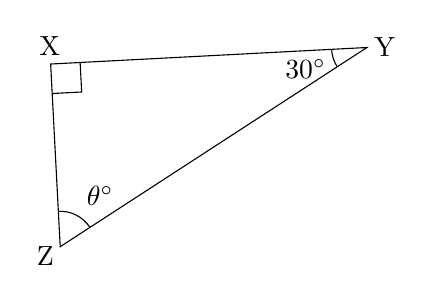
\begin{tikzpicture}[scale=1.5, baseline=(current bounding box.north)]
      \pgfmathsetmacro{\angleA}{60}
      \pgfmathsetmacro{\angleB}{30}
      \pgfmathsetmacro{\angleC}{90}
      \pgfmathsetmacro{\sideC}{3.0964220115623404}
      \pgfmathsetmacro{\rotationAngle}{33}
  
    
      \begin{scope}[rotate=\rotationAngle]
        \coordinate (A) at (0,0);
        \coordinate (B) at (\sideC,0);
        \coordinate (C) at (intersection cs: first line={(A)--($(A)+(\angleA:4cm)$)}, second line={(B)--($(B)+(180-\angleB:4cm)$)});
        \draw (A) -- (B) -- (C) -- cycle;
        
        % Mark angles with arcs
        \draw ($(A)!0.3cm!(B)$) arc [start angle=0, end angle=\angleA, radius=0.3cm];
        \draw ($(B)!0.3cm!(C)$) arc [start angle=180-\angleB, end angle=180, radius=0.3cm];
        % \draw ($(C)!0.3cm!(A)$) arc [start angle=180+\angleA, end angle=360-\angleB, radius=0.3cm];
        % rt angle mark at C
        % \tkzMarkRightAng0le(A,C,B); % uses \usepackage{tkz-euclide}
        \draw ($(C)!0.25cm!(A)$) -- ($(C)!0.25cm!(A)!0.25cm!90:(A)$) -- ($(C)!0.25cm!(B)$);
        %  The ($(C)!0.3cm!(A)!0.3cm!90:(A)$) syntax is used to specify a point that is 0.3cm away from the point ($(C)!0.3cm!(A)$) in a direction that is perpendicular to the line connecting points C and A. This is achieved by first specifying the point ($(C)!0.3cm!(A)$) and then rotating it by 90 degrees around point A using the !angle:anchor syntax.

        % Label angles
        \node at ($(A)!-0.15cm!(B)$) {Z};
        \node at ($(B)!-0.15cm!(C)$) {Y};
        \node at ($(C)!-0.15cm!(A)$) {X};
        
        % Mark angles in degrees
        \coordinate (midBC) at ($(B)!0.5!(C)$);
        \node at ($(A)!0.55cm!(midBC)$) {$\theta ^\circ$};
    
        \coordinate (midAC) at ($(A)!0.5!(C)$);
        \node at ($(B)!0.55cm!(midAC)$) {30$^\circ$};
    
        % \coordinate (midAB) at ($(A)!0.5!(B)$);
        % \node at ($(C)!0.55cm!(midAB)$) {90$^\circ$};
      
      \end{scope}
    \end{tikzpicture}
\end{minipage}%
\hfill
\begin{minipage}{0.4\textwidth}
    \begin{align*}
      \angle \text{Z} &= 90^\circ - \angle \text{Y} \\
      &= 90^\circ - 30^\circ  \\
      &= 60^\circ
    \end{align*}
\end{minipage}

\vspace{1cm}\begin{minipage}{0.55\textwidth}
  \refstepcounter{minipagecount}
  \noindent{(\theminipagecount)}\quad
  \begin{tikzpicture}[scale=1.5, baseline=(current bounding box.north)]
      \pgfmathsetmacro{\angleA}{36}
      \pgfmathsetmacro{\angleB}{54}
      \pgfmathsetmacro{\angleC}{90}
      \pgfmathsetmacro{\sideC}{3.6293803389156767}
      \pgfmathsetmacro{\rotationAngle}{121}
  
    
      \begin{scope}[rotate=\rotationAngle]
        \coordinate (A) at (0,0);
        \coordinate (B) at (\sideC,0);
        \coordinate (C) at (intersection cs: first line={(A)--($(A)+(\angleA:4cm)$)}, second line={(B)--($(B)+(180-\angleB:4cm)$)});
        \draw (A) -- (B) -- (C) -- cycle;
        
        % Mark angles with arcs
        \draw ($(A)!0.3cm!(B)$) arc [start angle=0, end angle=\angleA, radius=0.3cm];
        \draw ($(B)!0.3cm!(C)$) arc [start angle=180-\angleB, end angle=180, radius=0.3cm];
        % \draw ($(C)!0.3cm!(A)$) arc [start angle=180+\angleA, end angle=360-\angleB, radius=0.3cm];
        % rt angle mark at C
        % \tkzMarkRightAng0le(A,C,B); % uses \usepackage{tkz-euclide}
        \draw ($(C)!0.25cm!(A)$) -- ($(C)!0.25cm!(A)!0.25cm!90:(A)$) -- ($(C)!0.25cm!(B)$);
        %  The ($(C)!0.3cm!(A)!0.3cm!90:(A)$) syntax is used to specify a point that is 0.3cm away from the point ($(C)!0.3cm!(A)$) in a direction that is perpendicular to the line connecting points C and A. This is achieved by first specifying the point ($(C)!0.3cm!(A)$) and then rotating it by 90 degrees around point A using the !angle:anchor syntax.

        % Label angles
        \node at ($(A)!-0.15cm!(B)$) {Z};
        \node at ($(B)!-0.15cm!(C)$) {X};
        \node at ($(C)!-0.15cm!(A)$) {Y};
        
        % Mark angles in degrees
        \coordinate (midBC) at ($(B)!0.5!(C)$);
        \node at ($(A)!0.55cm!(midBC)$) {$\theta ^\circ$};
    
        \coordinate (midAC) at ($(A)!0.5!(C)$);
        \node at ($(B)!0.55cm!(midAC)$) {54$^\circ$};
    
        % \coordinate (midAB) at ($(A)!0.5!(B)$);
        % \node at ($(C)!0.55cm!(midAB)$) {90$^\circ$};
      
      \end{scope}
    \end{tikzpicture}
\end{minipage}%
\hfill
\begin{minipage}{0.4\textwidth}
    \begin{align*}
      \angle \text{Z} &= 90^\circ - \angle \text{X} \\
      &= 90^\circ - 54^\circ  \\
      &= 36^\circ
    \end{align*}
\end{minipage}

\vspace{1cm}\begin{minipage}{0.55\textwidth}
  \refstepcounter{minipagecount}
  \noindent{(\theminipagecount)}\quad
  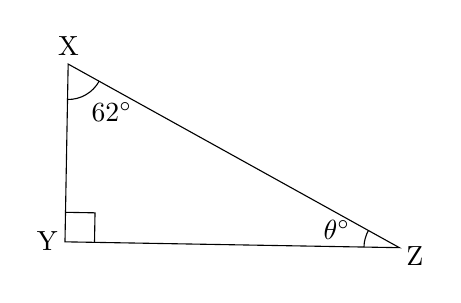
\begin{tikzpicture}[scale=1.5, baseline=(current bounding box.north)]
      \pgfmathsetmacro{\angleA}{28}
      \pgfmathsetmacro{\angleB}{62}
      \pgfmathsetmacro{\angleC}{90}
      \pgfmathsetmacro{\sideC}{3.2061834165776175}
      \pgfmathsetmacro{\rotationAngle}{151}
  
    
      \begin{scope}[rotate=\rotationAngle]
        \coordinate (A) at (0,0);
        \coordinate (B) at (\sideC,0);
        \coordinate (C) at (intersection cs: first line={(A)--($(A)+(\angleA:4cm)$)}, second line={(B)--($(B)+(180-\angleB:4cm)$)});
        \draw (A) -- (B) -- (C) -- cycle;
        
        % Mark angles with arcs
        \draw ($(A)!0.3cm!(B)$) arc [start angle=0, end angle=\angleA, radius=0.3cm];
        \draw ($(B)!0.3cm!(C)$) arc [start angle=180-\angleB, end angle=180, radius=0.3cm];
        % \draw ($(C)!0.3cm!(A)$) arc [start angle=180+\angleA, end angle=360-\angleB, radius=0.3cm];
        % rt angle mark at C
        % \tkzMarkRightAng0le(A,C,B); % uses \usepackage{tkz-euclide}
        \draw ($(C)!0.25cm!(A)$) -- ($(C)!0.25cm!(A)!0.25cm!90:(A)$) -- ($(C)!0.25cm!(B)$);
        %  The ($(C)!0.3cm!(A)!0.3cm!90:(A)$) syntax is used to specify a point that is 0.3cm away from the point ($(C)!0.3cm!(A)$) in a direction that is perpendicular to the line connecting points C and A. This is achieved by first specifying the point ($(C)!0.3cm!(A)$) and then rotating it by 90 degrees around point A using the !angle:anchor syntax.

        % Label angles
        \node at ($(A)!-0.15cm!(B)$) {Z};
        \node at ($(B)!-0.15cm!(C)$) {X};
        \node at ($(C)!-0.15cm!(A)$) {Y};
        
        % Mark angles in degrees
        \coordinate (midBC) at ($(B)!0.5!(C)$);
        \node at ($(A)!0.55cm!(midBC)$) {$\theta ^\circ$};
    
        \coordinate (midAC) at ($(A)!0.5!(C)$);
        \node at ($(B)!0.55cm!(midAC)$) {62$^\circ$};
    
        % \coordinate (midAB) at ($(A)!0.5!(B)$);
        % \node at ($(C)!0.55cm!(midAB)$) {90$^\circ$};
      
      \end{scope}
    \end{tikzpicture}
\end{minipage}%
\hfill
\begin{minipage}{0.4\textwidth}
    \begin{align*}
      \angle \text{Z} &= 90^\circ - \angle \text{X} \\
      &= 90^\circ - 62^\circ  \\
      &= 28^\circ
    \end{align*}
\end{minipage}

\vspace{1cm}\begin{minipage}{0.55\textwidth}
  \refstepcounter{minipagecount}
  \noindent{(\theminipagecount)}\quad
  \begin{tikzpicture}[scale=1.5, baseline=(current bounding box.north)]
      \pgfmathsetmacro{\angleA}{31}
      \pgfmathsetmacro{\angleB}{59}
      \pgfmathsetmacro{\angleC}{90}
      \pgfmathsetmacro{\sideC}{3.7600705052342533}
      \pgfmathsetmacro{\rotationAngle}{254}
  
    
      \begin{scope}[rotate=\rotationAngle]
        \coordinate (A) at (0,0);
        \coordinate (B) at (\sideC,0);
        \coordinate (C) at (intersection cs: first line={(A)--($(A)+(\angleA:4cm)$)}, second line={(B)--($(B)+(180-\angleB:4cm)$)});
        \draw (A) -- (B) -- (C) -- cycle;
        
        % Mark angles with arcs
        \draw ($(A)!0.3cm!(B)$) arc [start angle=0, end angle=\angleA, radius=0.3cm];
        \draw ($(B)!0.3cm!(C)$) arc [start angle=180-\angleB, end angle=180, radius=0.3cm];
        % \draw ($(C)!0.3cm!(A)$) arc [start angle=180+\angleA, end angle=360-\angleB, radius=0.3cm];
        % rt angle mark at C
        % \tkzMarkRightAng0le(A,C,B); % uses \usepackage{tkz-euclide}
        \draw ($(C)!0.25cm!(A)$) -- ($(C)!0.25cm!(A)!0.25cm!90:(A)$) -- ($(C)!0.25cm!(B)$);
        %  The ($(C)!0.3cm!(A)!0.3cm!90:(A)$) syntax is used to specify a point that is 0.3cm away from the point ($(C)!0.3cm!(A)$) in a direction that is perpendicular to the line connecting points C and A. This is achieved by first specifying the point ($(C)!0.3cm!(A)$) and then rotating it by 90 degrees around point A using the !angle:anchor syntax.

        % Label angles
        \node at ($(A)!-0.15cm!(B)$) {Z};
        \node at ($(B)!-0.15cm!(C)$) {X};
        \node at ($(C)!-0.15cm!(A)$) {Y};
        
        % Mark angles in degrees
        \coordinate (midBC) at ($(B)!0.5!(C)$);
        \node at ($(A)!0.55cm!(midBC)$) {$\theta ^\circ$};
    
        \coordinate (midAC) at ($(A)!0.5!(C)$);
        \node at ($(B)!0.55cm!(midAC)$) {59$^\circ$};
    
        % \coordinate (midAB) at ($(A)!0.5!(B)$);
        % \node at ($(C)!0.55cm!(midAB)$) {90$^\circ$};
      
      \end{scope}
    \end{tikzpicture}
\end{minipage}%
\hfill
\begin{minipage}{0.4\textwidth}
    \begin{align*}
      \angle \text{Z} &= 90^\circ - \angle \text{X} \\
      &= 90^\circ - 59^\circ  \\
      &= 31^\circ
    \end{align*}
\end{minipage}

\vspace{1cm}\begin{minipage}{0.55\textwidth}
  \refstepcounter{minipagecount}
  \noindent{(\theminipagecount)}\quad
  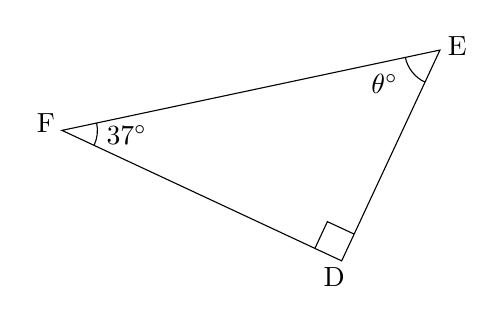
\begin{tikzpicture}[scale=1.5, baseline=(current bounding box.north)]
      \pgfmathsetmacro{\angleA}{53}
      \pgfmathsetmacro{\angleB}{37}
      \pgfmathsetmacro{\angleC}{90}
      \pgfmathsetmacro{\sideC}{3.271484601851906}
      \pgfmathsetmacro{\rotationAngle}{192}
  
    
      \begin{scope}[rotate=\rotationAngle]
        \coordinate (A) at (0,0);
        \coordinate (B) at (\sideC,0);
        \coordinate (C) at (intersection cs: first line={(A)--($(A)+(\angleA:4cm)$)}, second line={(B)--($(B)+(180-\angleB:4cm)$)});
        \draw (A) -- (B) -- (C) -- cycle;
        
        % Mark angles with arcs
        \draw ($(A)!0.3cm!(B)$) arc [start angle=0, end angle=\angleA, radius=0.3cm];
        \draw ($(B)!0.3cm!(C)$) arc [start angle=180-\angleB, end angle=180, radius=0.3cm];
        % \draw ($(C)!0.3cm!(A)$) arc [start angle=180+\angleA, end angle=360-\angleB, radius=0.3cm];
        % rt angle mark at C
        % \tkzMarkRightAng0le(A,C,B); % uses \usepackage{tkz-euclide}
        \draw ($(C)!0.25cm!(A)$) -- ($(C)!0.25cm!(A)!0.25cm!90:(A)$) -- ($(C)!0.25cm!(B)$);
        %  The ($(C)!0.3cm!(A)!0.3cm!90:(A)$) syntax is used to specify a point that is 0.3cm away from the point ($(C)!0.3cm!(A)$) in a direction that is perpendicular to the line connecting points C and A. This is achieved by first specifying the point ($(C)!0.3cm!(A)$) and then rotating it by 90 degrees around point A using the !angle:anchor syntax.

        % Label angles
        \node at ($(A)!-0.15cm!(B)$) {E};
        \node at ($(B)!-0.15cm!(C)$) {F};
        \node at ($(C)!-0.15cm!(A)$) {D};
        
        % Mark angles in degrees
        \coordinate (midBC) at ($(B)!0.5!(C)$);
        \node at ($(A)!0.55cm!(midBC)$) {$\theta ^\circ$};
    
        \coordinate (midAC) at ($(A)!0.5!(C)$);
        \node at ($(B)!0.55cm!(midAC)$) {37$^\circ$};
    
        % \coordinate (midAB) at ($(A)!0.5!(B)$);
        % \node at ($(C)!0.55cm!(midAB)$) {90$^\circ$};
      
      \end{scope}
    \end{tikzpicture}
\end{minipage}%
\hfill
\begin{minipage}{0.4\textwidth}
    \begin{align*}
      \angle \text{E} &= 90^\circ - \angle \text{F} \\
      &= 90^\circ - 37^\circ  \\
      &= 53^\circ
    \end{align*}
\end{minipage}

\vspace{1cm}\begin{minipage}{0.55\textwidth}
  \refstepcounter{minipagecount}
  \noindent{(\theminipagecount)}\quad
  \begin{tikzpicture}[scale=1.5, baseline=(current bounding box.north)]
      \pgfmathsetmacro{\angleA}{38}
      \pgfmathsetmacro{\angleB}{52}
      \pgfmathsetmacro{\angleC}{90}
      \pgfmathsetmacro{\sideC}{3.0185384286668215}
      \pgfmathsetmacro{\rotationAngle}{23}
  
    
      \begin{scope}[rotate=\rotationAngle]
        \coordinate (A) at (0,0);
        \coordinate (B) at (\sideC,0);
        \coordinate (C) at (intersection cs: first line={(A)--($(A)+(\angleA:4cm)$)}, second line={(B)--($(B)+(180-\angleB:4cm)$)});
        \draw (A) -- (B) -- (C) -- cycle;
        
        % Mark angles with arcs
        \draw ($(A)!0.3cm!(B)$) arc [start angle=0, end angle=\angleA, radius=0.3cm];
        \draw ($(B)!0.3cm!(C)$) arc [start angle=180-\angleB, end angle=180, radius=0.3cm];
        % \draw ($(C)!0.3cm!(A)$) arc [start angle=180+\angleA, end angle=360-\angleB, radius=0.3cm];
        % rt angle mark at C
        % \tkzMarkRightAng0le(A,C,B); % uses \usepackage{tkz-euclide}
        \draw ($(C)!0.25cm!(A)$) -- ($(C)!0.25cm!(A)!0.25cm!90:(A)$) -- ($(C)!0.25cm!(B)$);
        %  The ($(C)!0.3cm!(A)!0.3cm!90:(A)$) syntax is used to specify a point that is 0.3cm away from the point ($(C)!0.3cm!(A)$) in a direction that is perpendicular to the line connecting points C and A. This is achieved by first specifying the point ($(C)!0.3cm!(A)$) and then rotating it by 90 degrees around point A using the !angle:anchor syntax.

        % Label angles
        \node at ($(A)!-0.15cm!(B)$) {F};
        \node at ($(B)!-0.15cm!(C)$) {E};
        \node at ($(C)!-0.15cm!(A)$) {D};
        
        % Mark angles in degrees
        \coordinate (midBC) at ($(B)!0.5!(C)$);
        \node at ($(A)!0.55cm!(midBC)$) {$\theta ^\circ$};
    
        \coordinate (midAC) at ($(A)!0.5!(C)$);
        \node at ($(B)!0.55cm!(midAC)$) {52$^\circ$};
    
        % \coordinate (midAB) at ($(A)!0.5!(B)$);
        % \node at ($(C)!0.55cm!(midAB)$) {90$^\circ$};
      
      \end{scope}
    \end{tikzpicture}
\end{minipage}%
\hfill
\begin{minipage}{0.4\textwidth}
    \begin{align*}
      \angle \text{F} &= 90^\circ - \angle \text{E} \\
      &= 90^\circ - 52^\circ  \\
      &= 38^\circ
    \end{align*}
\end{minipage}

\vspace{1cm}\begin{minipage}{0.55\textwidth}
  \refstepcounter{minipagecount}
  \noindent{(\theminipagecount)}\quad
  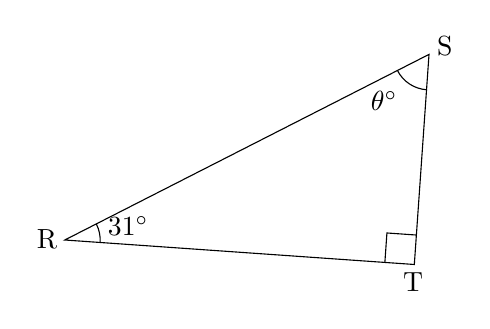
\begin{tikzpicture}[scale=1.5, baseline=(current bounding box.north)]
      \pgfmathsetmacro{\angleA}{59}
      \pgfmathsetmacro{\angleB}{31}
      \pgfmathsetmacro{\angleC}{90}
      \pgfmathsetmacro{\sideC}{3.4610105411796006}
      \pgfmathsetmacro{\rotationAngle}{207}
  
    
      \begin{scope}[rotate=\rotationAngle]
        \coordinate (A) at (0,0);
        \coordinate (B) at (\sideC,0);
        \coordinate (C) at (intersection cs: first line={(A)--($(A)+(\angleA:4cm)$)}, second line={(B)--($(B)+(180-\angleB:4cm)$)});
        \draw (A) -- (B) -- (C) -- cycle;
        
        % Mark angles with arcs
        \draw ($(A)!0.3cm!(B)$) arc [start angle=0, end angle=\angleA, radius=0.3cm];
        \draw ($(B)!0.3cm!(C)$) arc [start angle=180-\angleB, end angle=180, radius=0.3cm];
        % \draw ($(C)!0.3cm!(A)$) arc [start angle=180+\angleA, end angle=360-\angleB, radius=0.3cm];
        % rt angle mark at C
        % \tkzMarkRightAng0le(A,C,B); % uses \usepackage{tkz-euclide}
        \draw ($(C)!0.25cm!(A)$) -- ($(C)!0.25cm!(A)!0.25cm!90:(A)$) -- ($(C)!0.25cm!(B)$);
        %  The ($(C)!0.3cm!(A)!0.3cm!90:(A)$) syntax is used to specify a point that is 0.3cm away from the point ($(C)!0.3cm!(A)$) in a direction that is perpendicular to the line connecting points C and A. This is achieved by first specifying the point ($(C)!0.3cm!(A)$) and then rotating it by 90 degrees around point A using the !angle:anchor syntax.

        % Label angles
        \node at ($(A)!-0.15cm!(B)$) {S};
        \node at ($(B)!-0.15cm!(C)$) {R};
        \node at ($(C)!-0.15cm!(A)$) {T};
        
        % Mark angles in degrees
        \coordinate (midBC) at ($(B)!0.5!(C)$);
        \node at ($(A)!0.55cm!(midBC)$) {$\theta ^\circ$};
    
        \coordinate (midAC) at ($(A)!0.5!(C)$);
        \node at ($(B)!0.55cm!(midAC)$) {31$^\circ$};
    
        % \coordinate (midAB) at ($(A)!0.5!(B)$);
        % \node at ($(C)!0.55cm!(midAB)$) {90$^\circ$};
      
      \end{scope}
    \end{tikzpicture}
\end{minipage}%
\hfill
\begin{minipage}{0.4\textwidth}
    \begin{align*}
      \angle \text{S} &= 90^\circ - \angle \text{R} \\
      &= 90^\circ - 31^\circ  \\
      &= 59^\circ
    \end{align*}
\end{minipage}

\vspace{1cm}\begin{minipage}{0.55\textwidth}
  \refstepcounter{minipagecount}
  \noindent{(\theminipagecount)}\quad
  \begin{tikzpicture}[scale=1.5, baseline=(current bounding box.north)]
      \pgfmathsetmacro{\angleA}{65}
      \pgfmathsetmacro{\angleB}{25}
      \pgfmathsetmacro{\angleC}{90}
      \pgfmathsetmacro{\sideC}{3.2470835537890954}
      \pgfmathsetmacro{\rotationAngle}{339}
  
    
      \begin{scope}[rotate=\rotationAngle]
        \coordinate (A) at (0,0);
        \coordinate (B) at (\sideC,0);
        \coordinate (C) at (intersection cs: first line={(A)--($(A)+(\angleA:4cm)$)}, second line={(B)--($(B)+(180-\angleB:4cm)$)});
        \draw (A) -- (B) -- (C) -- cycle;
        
        % Mark angles with arcs
        \draw ($(A)!0.3cm!(B)$) arc [start angle=0, end angle=\angleA, radius=0.3cm];
        \draw ($(B)!0.3cm!(C)$) arc [start angle=180-\angleB, end angle=180, radius=0.3cm];
        % \draw ($(C)!0.3cm!(A)$) arc [start angle=180+\angleA, end angle=360-\angleB, radius=0.3cm];
        % rt angle mark at C
        % \tkzMarkRightAng0le(A,C,B); % uses \usepackage{tkz-euclide}
        \draw ($(C)!0.25cm!(A)$) -- ($(C)!0.25cm!(A)!0.25cm!90:(A)$) -- ($(C)!0.25cm!(B)$);
        %  The ($(C)!0.3cm!(A)!0.3cm!90:(A)$) syntax is used to specify a point that is 0.3cm away from the point ($(C)!0.3cm!(A)$) in a direction that is perpendicular to the line connecting points C and A. This is achieved by first specifying the point ($(C)!0.3cm!(A)$) and then rotating it by 90 degrees around point A using the !angle:anchor syntax.

        % Label angles
        \node at ($(A)!-0.15cm!(B)$) {A};
        \node at ($(B)!-0.15cm!(C)$) {B};
        \node at ($(C)!-0.15cm!(A)$) {C};
        
        % Mark angles in degrees
        \coordinate (midBC) at ($(B)!0.5!(C)$);
        \node at ($(A)!0.55cm!(midBC)$) {$\theta ^\circ$};
    
        \coordinate (midAC) at ($(A)!0.5!(C)$);
        \node at ($(B)!0.55cm!(midAC)$) {25$^\circ$};
    
        % \coordinate (midAB) at ($(A)!0.5!(B)$);
        % \node at ($(C)!0.55cm!(midAB)$) {90$^\circ$};
      
      \end{scope}
    \end{tikzpicture}
\end{minipage}%
\hfill
\begin{minipage}{0.4\textwidth}
    \begin{align*}
      \angle \text{A} &= 90^\circ - \angle \text{B} \\
      &= 90^\circ - 25^\circ  \\
      &= 65^\circ
    \end{align*}
\end{minipage}

\vspace{1cm}\begin{minipage}{0.55\textwidth}
  \refstepcounter{minipagecount}
  \noindent{(\theminipagecount)}\quad
  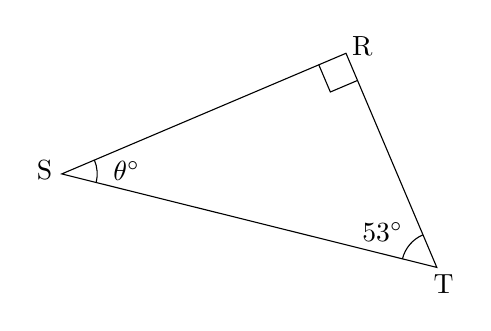
\begin{tikzpicture}[scale=1.5, baseline=(current bounding box.north)]
      \pgfmathsetmacro{\angleA}{37}
      \pgfmathsetmacro{\angleB}{53}
      \pgfmathsetmacro{\angleC}{90}
      \pgfmathsetmacro{\sideC}{3.2721154140703}
      \pgfmathsetmacro{\rotationAngle}{346}
  
    
      \begin{scope}[rotate=\rotationAngle]
        \coordinate (A) at (0,0);
        \coordinate (B) at (\sideC,0);
        \coordinate (C) at (intersection cs: first line={(A)--($(A)+(\angleA:4cm)$)}, second line={(B)--($(B)+(180-\angleB:4cm)$)});
        \draw (A) -- (B) -- (C) -- cycle;
        
        % Mark angles with arcs
        \draw ($(A)!0.3cm!(B)$) arc [start angle=0, end angle=\angleA, radius=0.3cm];
        \draw ($(B)!0.3cm!(C)$) arc [start angle=180-\angleB, end angle=180, radius=0.3cm];
        % \draw ($(C)!0.3cm!(A)$) arc [start angle=180+\angleA, end angle=360-\angleB, radius=0.3cm];
        % rt angle mark at C
        % \tkzMarkRightAng0le(A,C,B); % uses \usepackage{tkz-euclide}
        \draw ($(C)!0.25cm!(A)$) -- ($(C)!0.25cm!(A)!0.25cm!90:(A)$) -- ($(C)!0.25cm!(B)$);
        %  The ($(C)!0.3cm!(A)!0.3cm!90:(A)$) syntax is used to specify a point that is 0.3cm away from the point ($(C)!0.3cm!(A)$) in a direction that is perpendicular to the line connecting points C and A. This is achieved by first specifying the point ($(C)!0.3cm!(A)$) and then rotating it by 90 degrees around point A using the !angle:anchor syntax.

        % Label angles
        \node at ($(A)!-0.15cm!(B)$) {S};
        \node at ($(B)!-0.15cm!(C)$) {T};
        \node at ($(C)!-0.15cm!(A)$) {R};
        
        % Mark angles in degrees
        \coordinate (midBC) at ($(B)!0.5!(C)$);
        \node at ($(A)!0.55cm!(midBC)$) {$\theta ^\circ$};
    
        \coordinate (midAC) at ($(A)!0.5!(C)$);
        \node at ($(B)!0.55cm!(midAC)$) {53$^\circ$};
    
        % \coordinate (midAB) at ($(A)!0.5!(B)$);
        % \node at ($(C)!0.55cm!(midAB)$) {90$^\circ$};
      
      \end{scope}
    \end{tikzpicture}
\end{minipage}%
\hfill
\begin{minipage}{0.4\textwidth}
    \begin{align*}
      \angle \text{S} &= 90^\circ - \angle \text{T} \\
      &= 90^\circ - 53^\circ  \\
      &= 37^\circ
    \end{align*}
\end{minipage}

\vspace{1cm}\begin{minipage}{0.55\textwidth}
  \refstepcounter{minipagecount}
  \noindent{(\theminipagecount)}\quad
  \begin{tikzpicture}[scale=1.5, baseline=(current bounding box.north)]
      \pgfmathsetmacro{\angleA}{30}
      \pgfmathsetmacro{\angleB}{60}
      \pgfmathsetmacro{\angleC}{90}
      \pgfmathsetmacro{\sideC}{3.9654057526725754}
      \pgfmathsetmacro{\rotationAngle}{337}
  
    
      \begin{scope}[rotate=\rotationAngle]
        \coordinate (A) at (0,0);
        \coordinate (B) at (\sideC,0);
        \coordinate (C) at (intersection cs: first line={(A)--($(A)+(\angleA:4cm)$)}, second line={(B)--($(B)+(180-\angleB:4cm)$)});
        \draw (A) -- (B) -- (C) -- cycle;
        
        % Mark angles with arcs
        \draw ($(A)!0.3cm!(B)$) arc [start angle=0, end angle=\angleA, radius=0.3cm];
        \draw ($(B)!0.3cm!(C)$) arc [start angle=180-\angleB, end angle=180, radius=0.3cm];
        % \draw ($(C)!0.3cm!(A)$) arc [start angle=180+\angleA, end angle=360-\angleB, radius=0.3cm];
        % rt angle mark at C
        % \tkzMarkRightAng0le(A,C,B); % uses \usepackage{tkz-euclide}
        \draw ($(C)!0.25cm!(A)$) -- ($(C)!0.25cm!(A)!0.25cm!90:(A)$) -- ($(C)!0.25cm!(B)$);
        %  The ($(C)!0.3cm!(A)!0.3cm!90:(A)$) syntax is used to specify a point that is 0.3cm away from the point ($(C)!0.3cm!(A)$) in a direction that is perpendicular to the line connecting points C and A. This is achieved by first specifying the point ($(C)!0.3cm!(A)$) and then rotating it by 90 degrees around point A using the !angle:anchor syntax.

        % Label angles
        \node at ($(A)!-0.15cm!(B)$) {B};
        \node at ($(B)!-0.15cm!(C)$) {A};
        \node at ($(C)!-0.15cm!(A)$) {C};
        
        % Mark angles in degrees
        \coordinate (midBC) at ($(B)!0.5!(C)$);
        \node at ($(A)!0.55cm!(midBC)$) {$\theta ^\circ$};
    
        \coordinate (midAC) at ($(A)!0.5!(C)$);
        \node at ($(B)!0.55cm!(midAC)$) {60$^\circ$};
    
        % \coordinate (midAB) at ($(A)!0.5!(B)$);
        % \node at ($(C)!0.55cm!(midAB)$) {90$^\circ$};
      
      \end{scope}
    \end{tikzpicture}
\end{minipage}%
\hfill
\begin{minipage}{0.4\textwidth}
    \begin{align*}
      \angle \text{B} &= 90^\circ - \angle \text{A} \\
      &= 90^\circ - 60^\circ  \\
      &= 30^\circ
    \end{align*}
\end{minipage}

\vspace{1cm}\begin{minipage}{0.55\textwidth}
  \refstepcounter{minipagecount}
  \noindent{(\theminipagecount)}\quad
  \begin{tikzpicture}[scale=1.5, baseline=(current bounding box.north)]
      \pgfmathsetmacro{\angleA}{47}
      \pgfmathsetmacro{\angleB}{43}
      \pgfmathsetmacro{\angleC}{90}
      \pgfmathsetmacro{\sideC}{3.3819107371744677}
      \pgfmathsetmacro{\rotationAngle}{288}
  
    
      \begin{scope}[rotate=\rotationAngle]
        \coordinate (A) at (0,0);
        \coordinate (B) at (\sideC,0);
        \coordinate (C) at (intersection cs: first line={(A)--($(A)+(\angleA:4cm)$)}, second line={(B)--($(B)+(180-\angleB:4cm)$)});
        \draw (A) -- (B) -- (C) -- cycle;
        
        % Mark angles with arcs
        \draw ($(A)!0.3cm!(B)$) arc [start angle=0, end angle=\angleA, radius=0.3cm];
        \draw ($(B)!0.3cm!(C)$) arc [start angle=180-\angleB, end angle=180, radius=0.3cm];
        % \draw ($(C)!0.3cm!(A)$) arc [start angle=180+\angleA, end angle=360-\angleB, radius=0.3cm];
        % rt angle mark at C
        % \tkzMarkRightAng0le(A,C,B); % uses \usepackage{tkz-euclide}
        \draw ($(C)!0.25cm!(A)$) -- ($(C)!0.25cm!(A)!0.25cm!90:(A)$) -- ($(C)!0.25cm!(B)$);
        %  The ($(C)!0.3cm!(A)!0.3cm!90:(A)$) syntax is used to specify a point that is 0.3cm away from the point ($(C)!0.3cm!(A)$) in a direction that is perpendicular to the line connecting points C and A. This is achieved by first specifying the point ($(C)!0.3cm!(A)$) and then rotating it by 90 degrees around point A using the !angle:anchor syntax.

        % Label angles
        \node at ($(A)!-0.15cm!(B)$) {C};
        \node at ($(B)!-0.15cm!(C)$) {B};
        \node at ($(C)!-0.15cm!(A)$) {A};
        
        % Mark angles in degrees
        \coordinate (midBC) at ($(B)!0.5!(C)$);
        \node at ($(A)!0.55cm!(midBC)$) {$\theta ^\circ$};
    
        \coordinate (midAC) at ($(A)!0.5!(C)$);
        \node at ($(B)!0.55cm!(midAC)$) {43$^\circ$};
    
        % \coordinate (midAB) at ($(A)!0.5!(B)$);
        % \node at ($(C)!0.55cm!(midAB)$) {90$^\circ$};
      
      \end{scope}
    \end{tikzpicture}
\end{minipage}%
\hfill
\begin{minipage}{0.4\textwidth}
    \begin{align*}
      \angle \text{C} &= 90^\circ - \angle \text{B} \\
      &= 90^\circ - 43^\circ  \\
      &= 47^\circ
    \end{align*}
\end{minipage}

\vspace{1cm}\begin{minipage}{0.55\textwidth}
  \refstepcounter{minipagecount}
  \noindent{(\theminipagecount)}\quad
  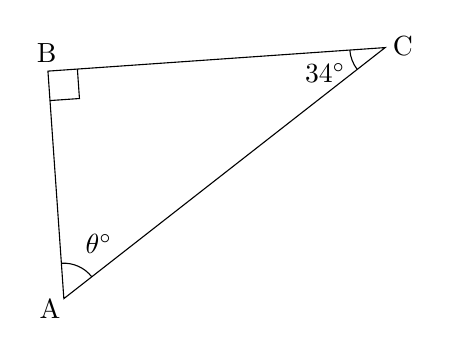
\begin{tikzpicture}[scale=1.5, baseline=(current bounding box.north)]
      \pgfmathsetmacro{\angleA}{56}
      \pgfmathsetmacro{\angleB}{34}
      \pgfmathsetmacro{\angleC}{90}
      \pgfmathsetmacro{\sideC}{3.45198317851618}
      \pgfmathsetmacro{\rotationAngle}{38}
  
    
      \begin{scope}[rotate=\rotationAngle]
        \coordinate (A) at (0,0);
        \coordinate (B) at (\sideC,0);
        \coordinate (C) at (intersection cs: first line={(A)--($(A)+(\angleA:4cm)$)}, second line={(B)--($(B)+(180-\angleB:4cm)$)});
        \draw (A) -- (B) -- (C) -- cycle;
        
        % Mark angles with arcs
        \draw ($(A)!0.3cm!(B)$) arc [start angle=0, end angle=\angleA, radius=0.3cm];
        \draw ($(B)!0.3cm!(C)$) arc [start angle=180-\angleB, end angle=180, radius=0.3cm];
        % \draw ($(C)!0.3cm!(A)$) arc [start angle=180+\angleA, end angle=360-\angleB, radius=0.3cm];
        % rt angle mark at C
        % \tkzMarkRightAng0le(A,C,B); % uses \usepackage{tkz-euclide}
        \draw ($(C)!0.25cm!(A)$) -- ($(C)!0.25cm!(A)!0.25cm!90:(A)$) -- ($(C)!0.25cm!(B)$);
        %  The ($(C)!0.3cm!(A)!0.3cm!90:(A)$) syntax is used to specify a point that is 0.3cm away from the point ($(C)!0.3cm!(A)$) in a direction that is perpendicular to the line connecting points C and A. This is achieved by first specifying the point ($(C)!0.3cm!(A)$) and then rotating it by 90 degrees around point A using the !angle:anchor syntax.

        % Label angles
        \node at ($(A)!-0.15cm!(B)$) {A};
        \node at ($(B)!-0.15cm!(C)$) {C};
        \node at ($(C)!-0.15cm!(A)$) {B};
        
        % Mark angles in degrees
        \coordinate (midBC) at ($(B)!0.5!(C)$);
        \node at ($(A)!0.55cm!(midBC)$) {$\theta ^\circ$};
    
        \coordinate (midAC) at ($(A)!0.5!(C)$);
        \node at ($(B)!0.55cm!(midAC)$) {34$^\circ$};
    
        % \coordinate (midAB) at ($(A)!0.5!(B)$);
        % \node at ($(C)!0.55cm!(midAB)$) {90$^\circ$};
      
      \end{scope}
    \end{tikzpicture}
\end{minipage}%
\hfill
\begin{minipage}{0.4\textwidth}
    \begin{align*}
      \angle \text{A} &= 90^\circ - \angle \text{C} \\
      &= 90^\circ - 34^\circ  \\
      &= 56^\circ
    \end{align*}
\end{minipage}

\vspace{1cm}\begin{minipage}{0.55\textwidth}
  \refstepcounter{minipagecount}
  \noindent{(\theminipagecount)}\quad
  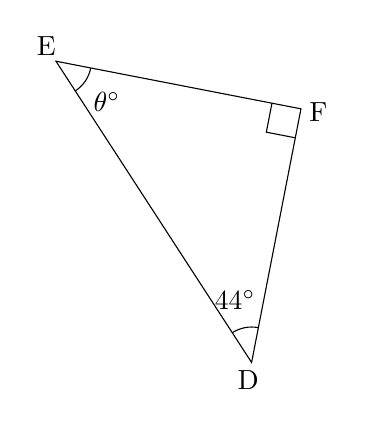
\begin{tikzpicture}[scale=1.5, baseline=(current bounding box.north)]
      \pgfmathsetmacro{\angleA}{46}
      \pgfmathsetmacro{\angleB}{44}
      \pgfmathsetmacro{\angleC}{90}
      \pgfmathsetmacro{\sideC}{3.0407600877613334}
      \pgfmathsetmacro{\rotationAngle}{303}
  
    
      \begin{scope}[rotate=\rotationAngle]
        \coordinate (A) at (0,0);
        \coordinate (B) at (\sideC,0);
        \coordinate (C) at (intersection cs: first line={(A)--($(A)+(\angleA:4cm)$)}, second line={(B)--($(B)+(180-\angleB:4cm)$)});
        \draw (A) -- (B) -- (C) -- cycle;
        
        % Mark angles with arcs
        \draw ($(A)!0.3cm!(B)$) arc [start angle=0, end angle=\angleA, radius=0.3cm];
        \draw ($(B)!0.3cm!(C)$) arc [start angle=180-\angleB, end angle=180, radius=0.3cm];
        % \draw ($(C)!0.3cm!(A)$) arc [start angle=180+\angleA, end angle=360-\angleB, radius=0.3cm];
        % rt angle mark at C
        % \tkzMarkRightAng0le(A,C,B); % uses \usepackage{tkz-euclide}
        \draw ($(C)!0.25cm!(A)$) -- ($(C)!0.25cm!(A)!0.25cm!90:(A)$) -- ($(C)!0.25cm!(B)$);
        %  The ($(C)!0.3cm!(A)!0.3cm!90:(A)$) syntax is used to specify a point that is 0.3cm away from the point ($(C)!0.3cm!(A)$) in a direction that is perpendicular to the line connecting points C and A. This is achieved by first specifying the point ($(C)!0.3cm!(A)$) and then rotating it by 90 degrees around point A using the !angle:anchor syntax.

        % Label angles
        \node at ($(A)!-0.15cm!(B)$) {E};
        \node at ($(B)!-0.15cm!(C)$) {D};
        \node at ($(C)!-0.15cm!(A)$) {F};
        
        % Mark angles in degrees
        \coordinate (midBC) at ($(B)!0.5!(C)$);
        \node at ($(A)!0.55cm!(midBC)$) {$\theta ^\circ$};
    
        \coordinate (midAC) at ($(A)!0.5!(C)$);
        \node at ($(B)!0.55cm!(midAC)$) {44$^\circ$};
    
        % \coordinate (midAB) at ($(A)!0.5!(B)$);
        % \node at ($(C)!0.55cm!(midAB)$) {90$^\circ$};
      
      \end{scope}
    \end{tikzpicture}
\end{minipage}%
\hfill
\begin{minipage}{0.4\textwidth}
    \begin{align*}
      \angle \text{E} &= 90^\circ - \angle \text{D} \\
      &= 90^\circ - 44^\circ  \\
      &= 46^\circ
    \end{align*}
\end{minipage}

\vspace{1cm}\begin{minipage}{0.55\textwidth}
  \refstepcounter{minipagecount}
  \noindent{(\theminipagecount)}\quad
  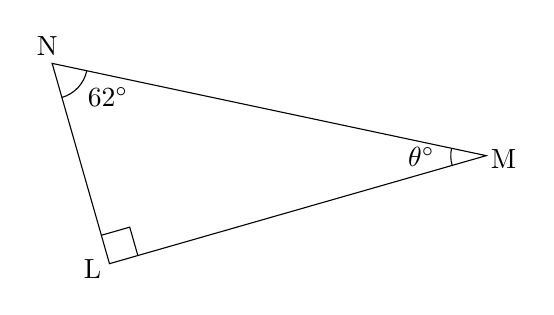
\begin{tikzpicture}[scale=1.5, baseline=(current bounding box.north)]
      \pgfmathsetmacro{\angleA}{28}
      \pgfmathsetmacro{\angleB}{62}
      \pgfmathsetmacro{\angleC}{90}
      \pgfmathsetmacro{\sideC}{3.7566686693490237}
      \pgfmathsetmacro{\rotationAngle}{168}
  
    
      \begin{scope}[rotate=\rotationAngle]
        \coordinate (A) at (0,0);
        \coordinate (B) at (\sideC,0);
        \coordinate (C) at (intersection cs: first line={(A)--($(A)+(\angleA:4cm)$)}, second line={(B)--($(B)+(180-\angleB:4cm)$)});
        \draw (A) -- (B) -- (C) -- cycle;
        
        % Mark angles with arcs
        \draw ($(A)!0.3cm!(B)$) arc [start angle=0, end angle=\angleA, radius=0.3cm];
        \draw ($(B)!0.3cm!(C)$) arc [start angle=180-\angleB, end angle=180, radius=0.3cm];
        % \draw ($(C)!0.3cm!(A)$) arc [start angle=180+\angleA, end angle=360-\angleB, radius=0.3cm];
        % rt angle mark at C
        % \tkzMarkRightAng0le(A,C,B); % uses \usepackage{tkz-euclide}
        \draw ($(C)!0.25cm!(A)$) -- ($(C)!0.25cm!(A)!0.25cm!90:(A)$) -- ($(C)!0.25cm!(B)$);
        %  The ($(C)!0.3cm!(A)!0.3cm!90:(A)$) syntax is used to specify a point that is 0.3cm away from the point ($(C)!0.3cm!(A)$) in a direction that is perpendicular to the line connecting points C and A. This is achieved by first specifying the point ($(C)!0.3cm!(A)$) and then rotating it by 90 degrees around point A using the !angle:anchor syntax.

        % Label angles
        \node at ($(A)!-0.15cm!(B)$) {M};
        \node at ($(B)!-0.15cm!(C)$) {N};
        \node at ($(C)!-0.15cm!(A)$) {L};
        
        % Mark angles in degrees
        \coordinate (midBC) at ($(B)!0.5!(C)$);
        \node at ($(A)!0.55cm!(midBC)$) {$\theta ^\circ$};
    
        \coordinate (midAC) at ($(A)!0.5!(C)$);
        \node at ($(B)!0.55cm!(midAC)$) {62$^\circ$};
    
        % \coordinate (midAB) at ($(A)!0.5!(B)$);
        % \node at ($(C)!0.55cm!(midAB)$) {90$^\circ$};
      
      \end{scope}
    \end{tikzpicture}
\end{minipage}%
\hfill
\begin{minipage}{0.4\textwidth}
    \begin{align*}
      \angle \text{M} &= 90^\circ - \angle \text{N} \\
      &= 90^\circ - 62^\circ  \\
      &= 28^\circ
    \end{align*}
\end{minipage}

\vspace{1cm}\begin{minipage}{0.55\textwidth}
  \refstepcounter{minipagecount}
  \noindent{(\theminipagecount)}\quad
  \begin{tikzpicture}[scale=1.5, baseline=(current bounding box.north)]
      \pgfmathsetmacro{\angleA}{50}
      \pgfmathsetmacro{\angleB}{40}
      \pgfmathsetmacro{\angleC}{90}
      \pgfmathsetmacro{\sideC}{3.8145629967019326}
      \pgfmathsetmacro{\rotationAngle}{159}
  
    
      \begin{scope}[rotate=\rotationAngle]
        \coordinate (A) at (0,0);
        \coordinate (B) at (\sideC,0);
        \coordinate (C) at (intersection cs: first line={(A)--($(A)+(\angleA:4cm)$)}, second line={(B)--($(B)+(180-\angleB:4cm)$)});
        \draw (A) -- (B) -- (C) -- cycle;
        
        % Mark angles with arcs
        \draw ($(A)!0.3cm!(B)$) arc [start angle=0, end angle=\angleA, radius=0.3cm];
        \draw ($(B)!0.3cm!(C)$) arc [start angle=180-\angleB, end angle=180, radius=0.3cm];
        % \draw ($(C)!0.3cm!(A)$) arc [start angle=180+\angleA, end angle=360-\angleB, radius=0.3cm];
        % rt angle mark at C
        % \tkzMarkRightAng0le(A,C,B); % uses \usepackage{tkz-euclide}
        \draw ($(C)!0.25cm!(A)$) -- ($(C)!0.25cm!(A)!0.25cm!90:(A)$) -- ($(C)!0.25cm!(B)$);
        %  The ($(C)!0.3cm!(A)!0.3cm!90:(A)$) syntax is used to specify a point that is 0.3cm away from the point ($(C)!0.3cm!(A)$) in a direction that is perpendicular to the line connecting points C and A. This is achieved by first specifying the point ($(C)!0.3cm!(A)$) and then rotating it by 90 degrees around point A using the !angle:anchor syntax.

        % Label angles
        \node at ($(A)!-0.15cm!(B)$) {N};
        \node at ($(B)!-0.15cm!(C)$) {M};
        \node at ($(C)!-0.15cm!(A)$) {L};
        
        % Mark angles in degrees
        \coordinate (midBC) at ($(B)!0.5!(C)$);
        \node at ($(A)!0.55cm!(midBC)$) {$\theta ^\circ$};
    
        \coordinate (midAC) at ($(A)!0.5!(C)$);
        \node at ($(B)!0.55cm!(midAC)$) {40$^\circ$};
    
        % \coordinate (midAB) at ($(A)!0.5!(B)$);
        % \node at ($(C)!0.55cm!(midAB)$) {90$^\circ$};
      
      \end{scope}
    \end{tikzpicture}
\end{minipage}%
\hfill
\begin{minipage}{0.4\textwidth}
    \begin{align*}
      \angle \text{N} &= 90^\circ - \angle \text{M} \\
      &= 90^\circ - 40^\circ  \\
      &= 50^\circ
    \end{align*}
\end{minipage}

\vspace{1cm}\begin{minipage}{0.55\textwidth}
  \refstepcounter{minipagecount}
  \noindent{(\theminipagecount)}\quad
  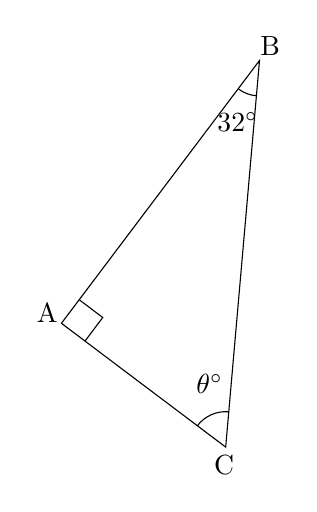
\begin{tikzpicture}[scale=1.5, baseline=(current bounding box.north)]
      \pgfmathsetmacro{\angleA}{58}
      \pgfmathsetmacro{\angleB}{32}
      \pgfmathsetmacro{\angleC}{90}
      \pgfmathsetmacro{\sideC}{3.285287098266962}
      \pgfmathsetmacro{\rotationAngle}{85}
  
    
      \begin{scope}[rotate=\rotationAngle]
        \coordinate (A) at (0,0);
        \coordinate (B) at (\sideC,0);
        \coordinate (C) at (intersection cs: first line={(A)--($(A)+(\angleA:4cm)$)}, second line={(B)--($(B)+(180-\angleB:4cm)$)});
        \draw (A) -- (B) -- (C) -- cycle;
        
        % Mark angles with arcs
        \draw ($(A)!0.3cm!(B)$) arc [start angle=0, end angle=\angleA, radius=0.3cm];
        \draw ($(B)!0.3cm!(C)$) arc [start angle=180-\angleB, end angle=180, radius=0.3cm];
        % \draw ($(C)!0.3cm!(A)$) arc [start angle=180+\angleA, end angle=360-\angleB, radius=0.3cm];
        % rt angle mark at C
        % \tkzMarkRightAng0le(A,C,B); % uses \usepackage{tkz-euclide}
        \draw ($(C)!0.25cm!(A)$) -- ($(C)!0.25cm!(A)!0.25cm!90:(A)$) -- ($(C)!0.25cm!(B)$);
        %  The ($(C)!0.3cm!(A)!0.3cm!90:(A)$) syntax is used to specify a point that is 0.3cm away from the point ($(C)!0.3cm!(A)$) in a direction that is perpendicular to the line connecting points C and A. This is achieved by first specifying the point ($(C)!0.3cm!(A)$) and then rotating it by 90 degrees around point A using the !angle:anchor syntax.

        % Label angles
        \node at ($(A)!-0.15cm!(B)$) {C};
        \node at ($(B)!-0.15cm!(C)$) {B};
        \node at ($(C)!-0.15cm!(A)$) {A};
        
        % Mark angles in degrees
        \coordinate (midBC) at ($(B)!0.5!(C)$);
        \node at ($(A)!0.55cm!(midBC)$) {$\theta ^\circ$};
    
        \coordinate (midAC) at ($(A)!0.5!(C)$);
        \node at ($(B)!0.55cm!(midAC)$) {32$^\circ$};
    
        % \coordinate (midAB) at ($(A)!0.5!(B)$);
        % \node at ($(C)!0.55cm!(midAB)$) {90$^\circ$};
      
      \end{scope}
    \end{tikzpicture}
\end{minipage}%
\hfill
\begin{minipage}{0.4\textwidth}
    \begin{align*}
      \angle \text{C} &= 90^\circ - \angle \text{B} \\
      &= 90^\circ - 32^\circ  \\
      &= 58^\circ
    \end{align*}
\end{minipage}

\vspace{1cm}\begin{minipage}{0.55\textwidth}
  \refstepcounter{minipagecount}
  \noindent{(\theminipagecount)}\quad
  \begin{tikzpicture}[scale=1.5, baseline=(current bounding box.north)]
      \pgfmathsetmacro{\angleA}{60}
      \pgfmathsetmacro{\angleB}{30}
      \pgfmathsetmacro{\angleC}{90}
      \pgfmathsetmacro{\sideC}{3.7924626745281858}
      \pgfmathsetmacro{\rotationAngle}{280}
  
    
      \begin{scope}[rotate=\rotationAngle]
        \coordinate (A) at (0,0);
        \coordinate (B) at (\sideC,0);
        \coordinate (C) at (intersection cs: first line={(A)--($(A)+(\angleA:4cm)$)}, second line={(B)--($(B)+(180-\angleB:4cm)$)});
        \draw (A) -- (B) -- (C) -- cycle;
        
        % Mark angles with arcs
        \draw ($(A)!0.3cm!(B)$) arc [start angle=0, end angle=\angleA, radius=0.3cm];
        \draw ($(B)!0.3cm!(C)$) arc [start angle=180-\angleB, end angle=180, radius=0.3cm];
        % \draw ($(C)!0.3cm!(A)$) arc [start angle=180+\angleA, end angle=360-\angleB, radius=0.3cm];
        % rt angle mark at C
        % \tkzMarkRightAng0le(A,C,B); % uses \usepackage{tkz-euclide}
        \draw ($(C)!0.25cm!(A)$) -- ($(C)!0.25cm!(A)!0.25cm!90:(A)$) -- ($(C)!0.25cm!(B)$);
        %  The ($(C)!0.3cm!(A)!0.3cm!90:(A)$) syntax is used to specify a point that is 0.3cm away from the point ($(C)!0.3cm!(A)$) in a direction that is perpendicular to the line connecting points C and A. This is achieved by first specifying the point ($(C)!0.3cm!(A)$) and then rotating it by 90 degrees around point A using the !angle:anchor syntax.

        % Label angles
        \node at ($(A)!-0.15cm!(B)$) {C};
        \node at ($(B)!-0.15cm!(C)$) {A};
        \node at ($(C)!-0.15cm!(A)$) {B};
        
        % Mark angles in degrees
        \coordinate (midBC) at ($(B)!0.5!(C)$);
        \node at ($(A)!0.55cm!(midBC)$) {$\theta ^\circ$};
    
        \coordinate (midAC) at ($(A)!0.5!(C)$);
        \node at ($(B)!0.55cm!(midAC)$) {30$^\circ$};
    
        % \coordinate (midAB) at ($(A)!0.5!(B)$);
        % \node at ($(C)!0.55cm!(midAB)$) {90$^\circ$};
      
      \end{scope}
    \end{tikzpicture}
\end{minipage}%
\hfill
\begin{minipage}{0.4\textwidth}
    \begin{align*}
      \angle \text{C} &= 90^\circ - \angle \text{A} \\
      &= 90^\circ - 30^\circ  \\
      &= 60^\circ
    \end{align*}
\end{minipage}

\vspace{1cm}

\end{document}
